\usepackage{tikz}
\usetikzlibrary{arrows,datavisualization.formats.functions,external}
\tikzexternalize[prefix=figures/]

\tikzset{
hollow node/.style={draw, circle,fill=white, minimum width=5pt, inner sep=0pt},
    black node/.style={draw, circle, fill=black, inner sep=0pt,
    minimum width=5pt}
}

\newcommand{\grapha}[3]{
\begin{tikzpicture}[scale=2]
  \datavisualization [school book axes,
    visualize as smooth line/.list={one},
    y axis={label={#3}},
    x axis={label={$t$}},
    one={style={black}},  
  ]

    data [set=one,format=function] {
        var x : interval [-#1:3];
        func y = exp(-2* (\value x+#1));
    };
    info{
    \node at (-#1+.4,0.4) [anchor=south west] {#2};
    };
    \draw [] (-#1,0) -- (-#1,1);
    
\end{tikzpicture}
}

\newcommand{\graphb}[6]{
\begin{tikzpicture}
    \datavisualization [school book axes,
    visualize as smooth line/.list={one,two},
    y axis={label={#6}, ticks={major={at={0}}}},
    x axis={label={$t$}, ticks={major={at={}}}},
    one={style={black}},
    two={style={black}}    
  ]

    data [set=one,format=function] {
        var x : interval [0:#1*3];
        func y = 2*exp(#4* \value x);
    }

    data [set=two,format=function] {
        var x : interval [-1.5*#1:0];
        func y = 2;
    };
    info{
    \node at (#1*1.5,1) [anchor=south west] {#5};
   \node at (0,2) [anchor=south east] {\small{$2$}};
   \node at (#2,0) [anchor=north] {\small{#2}};
   \node at (#3,0) [anchor=north east] {\small{#3}};
    };
    \draw [] (-1.5*#1,0) -- (-1.5*#1,2);
    \draw [] (3*#1,0) -- (3*#1,0.4462603203);
\end{tikzpicture}
}


\newcommand{\graphc}[5]{
\begin{tikzpicture}[scale=1.5]
    \datavisualization [school book axes,
    visualize as smooth line/.list={one,two},
    y axis={label={#4}},
    x axis={label={$t$}},
    one={style={black}}, 
    two={style={black}}, 
  ]

    data [set=one,format=function] {
        var x : interval [#1:#2];
        func y = exp(#3* \value x);
    };
    info{
    \node at (#1+2,0.3) [anchor=south west] {#5};
    };
    \ifnum#1>0
    \draw [] (1,0) -- (1,0.6065306597);
    \else
    \draw [] (-1,0) -- (-1,0.6065306597);
    \fi
\end{tikzpicture}
}


\newcommand{\evenodd}{
\begin{tikzpicture}[scale=2]
\datavisualization [school book axes,
    y axis={label={$x(t)$},ticks={minor={at={0,1,-1,0.5,-0.5}}},max value=1.5, min value=-1.5},
    x axis={label={$t$},ticks={major={at={1,-1}}},max value=1.5, min value=-1.5},
     ]
      info{
  \node at (0,0.5)  [anchor=west]{\small{$0.5$}};
  \node at (0,-0.5)  [anchor=east]{\small{$-0.5$}};
};
   \draw [ultra thick] (-1,0)--(-1,1); 
    \draw [ultra thick] (-1,1)--(0,0.5); 
   \draw [ultra thick] (0,0.5)--(0,-0.5);  
   \draw [ultra thick] (0,-0.5)--(1,0); 
\end{tikzpicture}
}

\newcommand{\evengrapha}{
\begin{tikzpicture}[scale=2]
\datavisualization [school book axes,
    y axis={label={$x(-t)$},ticks={minor={at={0,1,-1,0.5,-0.5}}},max value=1.5, min value=-1.5},
    x axis={label={$t$},ticks={major={at={1,-1}}},max value=1.5, min value=-1.5},
     ]
       info{
  \node at (0,0.5)  [anchor=east]{\small{$0.5$}};
  \node at (0,-0.5)  [anchor=west]{\small{$-0.5$}};
};
   \draw [ultra thick] (-1,0)--(0,-0.5); 
    \draw [ultra thick] (0,-0.5)--(0,0.5); 
   \draw [ultra thick] (0,0.5)--(1,1);  
   \draw [ultra thick] (1,1)--(1,0); 
\end{tikzpicture}
}
\newcommand{\evengraphb}{
\begin{tikzpicture}[scale=2]
\datavisualization [school book axes,
    y axis={label={$x(t)+x(-t)$},ticks={minor={at={0,1,-1,0.5,-0.5}}},max value=1.5, min value=-1.5},
    x axis={label={$t$},ticks={major={at={1,-1}}},max value=1.5, min value=-1.5},
     ];
   \draw [ultra thick] (-1,0)--(-1,1);  
   \draw [ultra thick] (-1,1)--(0,0); 
    \draw [ultra thick] (0,0)--(1,1); 
   \draw [ultra thick] (1,1)--(1,0); 
\end{tikzpicture}
}
\newcommand{\evengraphc}{
\begin{tikzpicture}[scale=2]
\datavisualization [school book axes,
    y axis={label={$x_e=\frac{x(t)+x(-t)}{2}$},ticks={major={at={0,1,-1,0.5,-0.5}}},max value=1.5, min value=-1.5},
    x axis={label={$t$},ticks={major={at={1,-1}}},max value=1.5, min value=-1.5},
     ];
   \draw [ultra thick] (-1,0)--(-1,0.5);  
   \draw [ultra thick] (-1,0.5)--(0,0); 
    \draw [ultra thick] (0,0)--(1,0.5); 
   \draw [ultra thick] (1,0.5)--(1,0); 
\end{tikzpicture}
}
\newcommand{\oddgrapha}{
\begin{tikzpicture}[scale=1.5]
\datavisualization [school book axes,
    y axis={label={$-x(-t)$},ticks={minor={at={0,1,-1,0.5,-0.5}}},max value=1.5, min value=-1.5},
    x axis={label={$t$},ticks={major={at={-1}}},max value=1.5, min value=-1.5},
     ]
       info{
  \node at (0,0.5)  [anchor=west]{\small{$0.5$}};
  \node at (0,-0.5)  [anchor=east]{\small{$-0.5$}};
  \node at (1,0)  [anchor=south]{\small{$1$}};
};
   \draw [ultra thick] (-1,0)--(0,0.5); 
    \draw [ultra thick] (0,0.5)--(0,-0.5); 
   \draw [ultra thick] (0,-0.5)--(1,-1);  
   \draw [ultra thick] (1,-1)--(1,0); 
\end{tikzpicture}
}
\newcommand{\oddgraphb}{
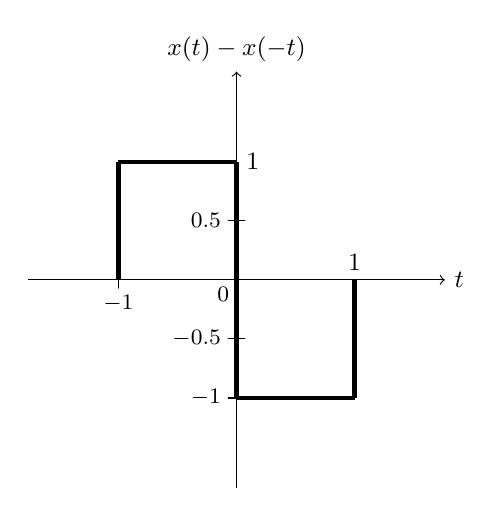
\begin{tikzpicture}[scale=1.5]
\datavisualization [school book axes,
    y axis={label={$x(t)-x(-t)$},ticks={major={at={0,-1,0.5,-0.5}}},max value=1.5, min value=-1.5},
    x axis={label={$t$},ticks={major={at={-1}}},max value=1.5, min value=-1.5},
     ]
       info{
  \node at (0,1)  [anchor=west]{\small{$1$}};
  \node at (1,0)  [anchor=south]{\small{$1$}};
};
   \draw [ultra thick] (-1,0)--(-1,1); 
    \draw [ultra thick] (-1,1)--(0,1); 
   \draw [ultra thick] (0,1)--(0,-1);  
   \draw [ultra thick] (0,-1)--(1,-1); 
   \draw [ultra thick] (1,-1)--(1,0); 
\end{tikzpicture}
}
\newcommand{\oddgraphc}{
\begin{tikzpicture}[scale=1.5]
\datavisualization [school book axes,
    y axis={label={$x_o=\frac{x(t)-x(-t)}{2}$},ticks={minor={at={0,1,-1,0.5,-0.5}}},max value=1.5, min value=-1.5},
    x axis={label={$t$},ticks={major={at={-1}}},max value=1.5, min value=-1.5},
     ]
       info{
  \node at (0,0.5)  [anchor=west]{\small{$0.5$}};
  \node at (0,-0.5)  [anchor=east]{\small{$-0.5$}};
  \node at (1,0)  [anchor=south]{\small{$1$}};
};
   \draw [ultra thick] (-1,0)--(-1,0.5); 
    \draw [ultra thick] (-1,0.5)--(0,0.5); 
   \draw [ultra thick] (0,0.5)--(0,-0.5);  
   \draw [ultra thick] (0,-0.5)--(1,-0.5); 
   \draw [ultra thick] (1,-0.5)--(1,0); 
\end{tikzpicture}
}

\newcommand{\rectContinuous}{
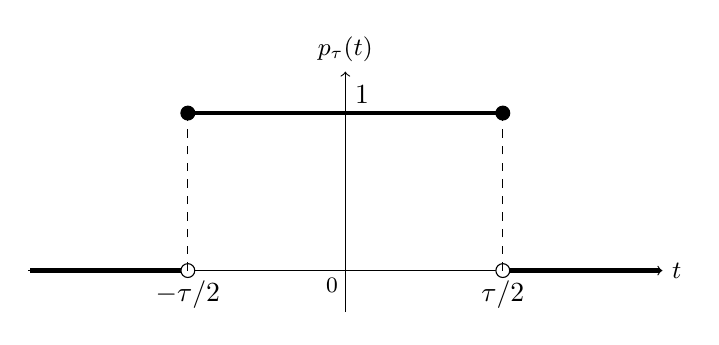
\begin{tikzpicture}[scale=2]
  \datavisualization [school book axes,
    visualize as smooth line/.list={one,two,three},
    y axis={label={$p_\tau(t)$},ticks={major={at={0}}},max value=1, min value=0},
    x axis={label={$t$},ticks={major={at={}}},max value=1.75, min value=-1.75},
    one={style={black, ultra thick}},
    two={style={black, ultra thick}}, 
    three={style={black, ultra thick}}, 
  ]

    data [set=one,format=function] {
        var x : interval [-1:1];
        func y = 1;
    }
    data [set=two,format=function] {
        var x : interval [-2:-1];
        func y = 0;
    }
    data [set=three,format=function] {
        var x : interval [1:2];
        func y = 0;
    };
    info{
  \node at (1,0) [anchor=north] {$\tau/2$};
  \node at (-1,0) [anchor=north] {$-\tau/2$};
  \node at (0,1) [anchor=south west] {$1$};
  \node at (1,0)[hollow node]  {};
  \node at (-1,0)[hollow node]  {};
  \node at (1,1)[black node]  {};
  \node at (-1,1)[black node]  {};
    };
    
    \draw [dashed] (1,0) -- (1,1);
     \draw [dashed] (-1,0) -- (-1,1);
     
\end{tikzpicture}
}

\newcommand{\rectDiscrete}{
\begin{tikzpicture}[scale=2]
  \datavisualization [school book axes,
    y axis={label={$p_\tau[n]$},ticks={major={at={0}}}, max value=1, min value=0},
    x axis={label={$n$},ticks={major={at={}}},max value=2, min value=-2},
  ]

    info{
  \node at (1,0) [anchor=north] {$m/2$};
  \node at (-1,0) [anchor=north] {$-m/2$};
  \node at (0,1) [anchor=south west] {$1$};
  \node at (1,0)[hollow node]  {};
  \node at (-1,0)[hollow node]  {};
\foreach \position in {(-2,0),(-1.5,0),(-1,1),(-0.5,1),(0,1),(0.5,1),(1,1),(1.5,0),(2,0)}
\node at \position [black node]{};
    };
    
    \draw [dashed] (1,0) -- (1,1);
    \draw [dashed] (-1,0) -- (-1,1);
     
\end{tikzpicture}
}

\newcommand{\rampContinuous}{
\begin{tikzpicture}[scale=2]
  \datavisualization [school book axes,
    y axis={label={$r(t)$},ticks={major={at={0}}}, max value=2, min value=0},
    x axis={label={$t$},ticks={major={at={}}},max value=2 , min value=-1.75},
  ];
    
    \draw [ultra thick, ->] (0,0) -- (1.75,1.75);
    \draw [ultra thick] (-2,0) -- (0,0);
     
\end{tikzpicture}
}
\newcommand{\rampDiscrete}{
\begin{tikzpicture}[scale=2]
  \datavisualization [school book axes,
    y axis={label={$r[n]$},ticks={major={at={0}}}, max value=2, min value=0},
    x axis={label={$n$},ticks={major={at={1,2,-1,-2}}},max value=2 , min value=-1.75},
  ];
    info{
\foreach \position in {(-2,0),(-1,0),(0,0),(1,1),(2,2)}
\node at \position [black node]{};
    };
\end{tikzpicture}
}

\newcommand{\signumContinuous}{
\begin{tikzpicture}[scale=2]
  \datavisualization [school book axes,
    y axis={label={$sgn(t)$},ticks={major={at={}}}, max value=1, min value=-1},
    x axis={label={$t$},ticks={major={at={}}},max value=2, min value=-2},
  ]

    info{
  \node at (0,-1)[hollow node]  {};
  \node at (0,1)[hollow node]  {};
  \node at (0,0)[black node]  {};
  \node at (0,1)  [anchor=east]{$1$};
  \node at (0,-1)  [anchor=west]{$-1$};
};
    
    \draw [ultra thick] (0,1) -- (2,1);
    \draw [ultra thick] (0,-1) -- (-2,-1);
     
\end{tikzpicture}
}
\newcommand{\signumDiscrete}{
\begin{tikzpicture}[scale=2]
  \datavisualization [school book axes,
    y axis={label={$sgn[n]$},ticks={major={at={}}}, max value=1, min value=-1},
    x axis={label={$n$},ticks={major={at={}}},max value=2, min value=-2},
  ]
  
    info{
   \node at (0,1)  [anchor=east]{$1$};
   \node at (0,-1)  [anchor=west]{$-1$};
   \foreach \position in {(-2,-1),(-1,-1),(0,0),(1,1),(2,1)}
\node at \position [black node]{};
};
    
    \draw [dashed] (0,1) -- (2,1);
    \draw [dashed] (0,-1) -- (-2,-1);
     
\end{tikzpicture}
}